\documentclass[usenames,dvipsnames]{beamer}

\mode<presentation>
{
  \usetheme{CambridgeUS}
  \usecolortheme{orchid}
  \setbeamercovered{transparent}
  \useinnertheme{rectangles}
  \setbeamertemplate{navigation symbols}{}
  \usefonttheme[onlymath]{serif}
  \setbeamercolor{title}{bg=alerted text.fg!85!black, fg=white}
  \setbeamercolor{item projected}{bg=alerted text.fg!85!black}
  \setbeamertemplate{enumerate items}[default]
  \setbeamercolor{local structure}{fg=alerted text.fg!85!black}
  \setbeamersize{text margin left=0.2cm,text margin right=0.2cm}
}

\newcommand\Shorter[2][1]{%
\makebox[\linewidth][c]{%
  \begin{minipage}{\dimexpr\textwidth+#1\relax}
  \raggedright#2
  \end{minipage}%
  }%
}
\usepackage[english]{babel}
\usepackage[utf8]{inputenc}
\usepackage[T1]{fontenc}
\usepackage{lmodern}
\usepackage{pifont}
\usepackage{mathrsfs}
\usepackage{amsmath}
\usepackage{bm}
\usepackage{caption}
\usepackage{subcaption}
\usepackage{outlines}
\usepackage{booktabs}
\usepackage{minted}
\usepackage[listings, minted]{tcolorbox}
\tcbset{left=2mm}
\usepackage[%
autocite     = plain,
doi          = true,
url          = true,
giveninits   = true,
hyperref     = true,
backref      = true,
maxbibnames  = 99,
maxcitenames = 99,
sortcites    = true,
style        = authoryear,
]{biblatex}

\addbibresource{presentation.bib}

\newcommand{\fakeimage}{{\fboxsep=-\fboxrule\fbox{\rule{0pt}{3cm}\hspace{4cm}}}}

\usepackage{tikz}
\usetikzlibrary{quotes}
\usetikzlibrary{bayesnet}
\usetikzlibrary{arrows,calc,positioning,decorations.pathreplacing}
\tikzset{
  >=stealth',
  punkt/.style={
    circle,
    draw=black, thick,
    minimum height=1.75em,
    inner sep=0pt,
    text centered},
  pil/.style={
    ->,
    thick}
}

\definecolor{isabelline}{rgb}{0.96, 0.94, 0.93}
\definecolor{palesilver}{rgb}{0.79, 0.75, 0.73}
\definecolor{hdblue}{HTML}{3366cc}
\hypersetup{colorlinks,linkcolor=,urlcolor=hdblue, citecolor=hdblue}

\setminted{highlightcolor=black!5, linenos}
\setminted{style=emacs}
\setminted{bgcolor=isabelline}
\setminted{fontsize=\fontsize{10}{1}\selectfont}
\setminted{highlightcolor=palesilver}
\setminted{numbers=left,autogobble,numbersep=0.1em}
\renewcommand{\theFancyVerbLine}{{\fontsize{6}{6}\selectfont \arabic{FancyVerbLine}}}

\newcommand{\xmark}{\ding{55}}
\newcommand{\highlight}[1]{%
  \colorbox{blue!20}{$\displaystyle#1$}}


\def\ci{\perp\!\!\!\perp}
\makeatletter
\newcommand*{\indep}{%
  \mathbin{%
    \mathpalette{\@indep}{}%
  }%
}
\newcommand*{\nindep}{%
\mathbin{%                   % The final symbol is a binary math operator
  \mathpalette{\@indep}{\not}% \mathpalette helps for the adaptation
  % of the symbol to the different math styles.
}%
}
\def\layersep{.38cm}
\def\inlsep{.4}
\newcommand*{\@indep}[2]{%
% #1: math style
% #2: empty or \not
  \sbox0{$#1\perp\m@th$}%        box 0 contains \perp symbol
  \sbox2{$#1=$}%                 box 2 for the height of =
  \sbox4{$#1\vcenter{}$}%        box 4 for the height of the math axis
  \rlap{\copy0}%                 first \perp
  \dimen@=\dimexpr\ht2-\ht4-.2pt\relax
  % The equals symbol is centered around the math axis.
  % The following equations are used to calculate the
  % right shift of the second \perp:
  % [1] ht(equals) - ht(math_axis) = line_width + 0.5 gap
  % [2] right_shift(second_perp) = line_width + gap
  % The line width is approximated by the default line width of 0.4pt
  \kern\dimen@
  {#2}%
  % {\not} in case of \nindep;
  % the braces convert the relational symbol \not to an ordinary
  % math object without additional horizontal spacing.
  \kern\dimen@
  \copy0 %                       second \perp
}
\makeatother


\title[PPL]{Probabilistic Programming Languages}

% \subtitle
% {Presentation Subtitle} % (optional)

\author[Dogan]
{%
\texorpdfstring{
  \begin{columns}
    \column{.85\linewidth}
    \centering
    Haluk Dogan\\
    \url{https://haluk.github.io/}\\
    \href{mailto:hdogan@vivaldi.net}{hdogan@vivaldi.net} \\
  \end{columns}
}
{Dogan}
}
\institute[SBBI {\fontsize{5}{6}\selectfont @} CSE {\fontsize{5}{6}\selectfont
  @} UNL] % (optional, but mostly needed)
{
  Department of Computer Science\\
  University of Nebraska-Lincoln
}

\date[\today] % (optional)
{\today\\
  \vspace{0.5cm}
  \begin{tiny}Some slides copied from \\
    Dr. Frank Wood,  University of Oxford
  \end{tiny}
}

\subject{Talks}

\pgfdeclareimage[height=0.5cm]{university-logo}{figures/logo}
\logo{\pgfuseimage{university-logo}}

\begin{document}

\begin{frame}[noframenumbering,plain]
  \titlepage{}
\end{frame}

%\section{Introduction}\label{sec:introduction}
\begin{frame}
  \frametitle{Probabilistic Programming Languages (PPL)}
  \begin{figure}[ht]
    \centering
    \includegraphics[width=0.65\textwidth,keepaspectratio]{figures/pplvenn.pdf}
    \caption*{\label{fig:ppl-venn}}
  \end{figure}
\end{frame}
\begin{frame}
  \frametitle{What and Why}
  \begin{alertblock}{Probabilistic Programming is Not}
    About writing software that behaves probabilistically
    \begin{itemize}
      \item \textrm{rand} as in cryptographic key generator
    \end{itemize}
  \end{alertblock}
  \begin{exampleblock}{Probabilistic Programming Is}
    \begin{itemize}
      \item A tool for statistical modeling
      \item \textrm{rand} and a great big pile of related tools
    \end{itemize}
  \end{exampleblock}
  \begin{block}{Goal}
    Bring the old and powerful magic of programming
    languages, which you already know and love, to the world of statistics.
  \end{block}
\end{frame}
\begin{frame}
  \frametitle{Intuition}
  \begin{figure}[ht]
    \centering
    \includegraphics[height=0.7\textheight,keepaspectratio]{figures/ppl_similarity.pdf}
    \caption*{\label{fig:ppl-similarity}}
  \end{figure}
\end{frame}
\begin{frame}
  \frametitle{The Way Machine Learning Is}
  \begin{figure}[ht]
    \includegraphics[width=1\textwidth,keepaspectratio]{figures/ml_current.pdf}
    \caption*{\label{fig:ml-current}}
  \end{figure}
\end{frame}
\begin{frame}
  \frametitle{The Way Machine Learning Will Be }
  \begin{figure}[ht]
    \includegraphics[width=1\textwidth,keepaspectratio]{figures/ml_future.pdf}
    \caption*{\label{fig:ml-future}}
  \end{figure}
\end{frame}
\begin{frame}
  \frametitle{PL Concepts to Statistical Modeling}
  \begin{center}
    \LARGE Abstraction
  \end{center}
  \vspace{-1cm}
  \begin{columns}
    \begin{column}{.48\textwidth}
      \begin{figure}[ht]
        \centering
        \includegraphics[width=1.0\textwidth,height=0.65\textheight]{figures/abstraction1.png}
        \caption*{\label{fig:abstration1}}
      \end{figure}
    \end{column}
    \begin{column}{.48\textwidth}
      \begin{figure}[ht]
        \centering
        \includegraphics[width=1.0\textwidth,height=0.65\textheight]{figures/abstraction2.png}
        \caption*{\label{fig:abstration2}}
      \end{figure}
    \end{column}
  \end{columns}
\end{frame}
\begin{frame}
  \frametitle{PL Concepts to Statistical Modeling (cont'd)}
  \begin{figure}[ht]
    \centering
    \includegraphics[width=1.0\textwidth,height=0.75\textheight]{figures/reuse.png}
    \caption*{\label{fig:reuse}}
  \end{figure}
\end{frame}
\begin{frame}
  \frametitle{PL Concepts to Statistical Modeling (cont'd)}
  \begin{center}
    \LARGE Simplicity
  \end{center}
  \vspace{-0.5cm}
  \begin{figure}[ht]
    \centering
    \includegraphics[width=1.0\textwidth,height=0.65\textheight]{figures/simplicity.png}
    \caption*{\label{fig:simplicity}}
  \end{figure}
\end{frame}
\begin{frame}
  \frametitle{Paper Recommender System\footnotemark}
  \begin{columns}
    \begin{column}{.48\textwidth}
      \begin{figure}[ht]
        \centering
        \includegraphics[width=1.0\textwidth,keepaspectratio]{figures/ex-problem.pdf}
        \caption*{\label{fig:ex-problem}}
      \end{figure}
    \end{column}
    \begin{column}{.48\textwidth}
      \begin{itemize}
        \item CS 4110: PL
        \item CS 4780: ML
        \item CS 4242: PPL
        \item Taking 4780 means interested in statistics?
        \item Taking 4242 and neither 4110 nor 4780 means 50/50 PL/stats?
      \end{itemize}
    \end{column}
  \end{columns}
  \footnotetext[1]{\url{http://adriansampson.net/doc/ppl.html}}
\end{frame}
\begin{frame}
  \frametitle{Paper Recommender System (cont'd)}
  \begin{columns}[t]
    \begin{column}{.48\textwidth}
      \begin{figure}[ht]
        \centering
        \includegraphics[width=0.7\textheight,keepaspectratio]{figures/ex-model-full.pdf}
        \caption*{\label{fig:ex-causal-full}}
      \end{figure}
    \end{column}
    \begin{column}{.48\textwidth}
      \begin{figure}[ht]
        \centering
        \includegraphics[width=0.7\textheight,keepaspectratio]{figures/ex-model-out.pdf}
        \caption*{\label{fig:ex-causal-out}}
      \end{figure}
    \end{column}
  \end{columns}
\end{frame}
\begin{frame}
  \frametitle{Paper Recommender System (cont'd)}
  \vspace{-0.8cm}
  \begin{columns}[t]
    \begin{column}{.48\textwidth}
      \begin{align*}
        &\text{Pr} [ A_\text{4780} | I_\text{stats} \wedge B ] = 0.3 \\
        &\text{Pr} [ A_\text{4780} | I_\text{stats} \wedge \neg B ] = 0.8 \\
        &\text{Pr} [ A_\text{4780} | \neg I_\text{stats} ] = 0.1 \\
        &\vdots \\
        &\text{Pr} [ A_\text{4242} | I_\text{stats} \wedge I_\text{PL} ] = 0.3 \\
        &\text{Pr} [ A_\text{4242} | I_\text{stats} \wedge I_\text{PL} \wedge \neg B ] = 0.8 \\
        &\text{Pr} [ A_\text{4242} | \neg (I_\text{stats} \vee I_\text{PL}) ] = 0.1 \\
        &\vdots \\
        &R_1 \sim I_\text{PL} \wedge I_\text{stats} \\
        &R_2 \sim I_\text{PL} \\
        &R_3 \sim I_\text{stats} \\
      \end{align*}
    \end{column}
    \begin{column}{.48\textwidth}
      \begin{itemize}
        \item no abstraction
        \item no reuse
        \item no descriptive variable names,
        \item no comments
        \item no debugger
        \item no type systems
      \end{itemize}
    \end{column}
  \end{columns}
\end{frame}
\begin{frame}[fragile]
  \frametitle{Basic Concepts}
  Random primitives
  \begin{minted}{js}
      var b = flip(0.5);
      b ? "yes" : "no"
  \end{minted}
  \begin{columns}[t]
    \begin{column}{0.60\textwidth}
      \inputminted[autogobble]{js}{src/enumerate.wppl}
    \end{column}
    \begin{column}{.36\textwidth}
      \begin{figure}[ht]
        \centering
        \includegraphics[width=1\textwidth,keepaspectratio]{figures/enumerate.png}
        \caption*{\label{fig:enumerate}}
      \end{figure}
    \end{column}
  \end{columns}
\end{frame}
\begin{frame}[fragile]
  \frametitle{Basic Concepts (cont'd)}
  \vspace{-1cm}
  \begin{columns}[t]
    \begin{column}{.6\textwidth}
      \inputminted[autogobble,fontsize=\fontsize{4.5}{4.5}\selectfont]{js}{src/model.wppl}
    \end{column}
    \begin{column}{.36\textwidth}
      \begin{figure}[ht]
        \centering
        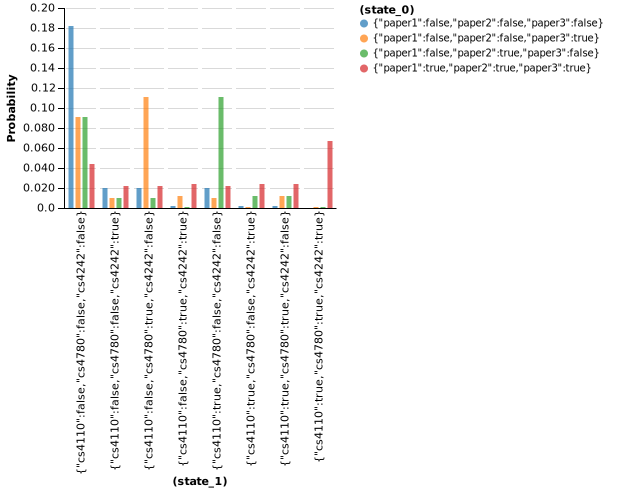
\includegraphics[width=1\textwidth,height=0.6\textheight]{figures/model.png}
        \caption*{\label{fig:modeldist}}
      \end{figure}
    \end{column}
  \end{columns}
\end{frame}
\begin{frame}[fragile]
  \frametitle{Basic Concepts (cont'd)}
  Conditioning
  \begin{columns}[t]
    \begin{column}{.65\textwidth}
      \inputminted[fontsize=\fontsize{7}{7}\selectfont]{js}{src/roll4.wppl}
    \end{column}
    \begin{column}{.31\textwidth}
      \begin{figure}[ht]
        \centering
        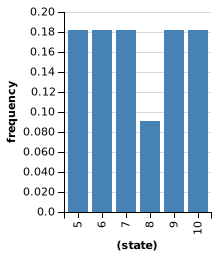
\includegraphics[width=1\textwidth,height=0.6\textheight]{figures/roll4.png}
        \caption*{\label{fig:roll4}}
      \end{figure}
    \end{column}
  \end{columns}
\end{frame}
\begin{frame}[fragile]
  \frametitle{Basic Concepts (cont'd)}
  \begin{columns}[t]
    \begin{column}{.65\textwidth}
      \inputminted[fontsize=\fontsize{7}{7}\selectfont]{js}{src/roll10.wppl}
    \end{column}
    \begin{column}{.31\textwidth}
      \begin{figure}[ht]
        \centering
        \includegraphics[width=1\textwidth,height=0.6\textheight]{figures/roll10.png}
        \caption*{\label{fig:roll10}}
      \end{figure}
    \end{column}
  \end{columns}
\end{frame}
\begin{frame}[fragile]
  \frametitle{Actually Recommending Papers Example}
  Attend CS 4110 (PL), and CS 4242 (PPL), but not the CS 4780 (ML)
  \begin{columns}[t]
    \begin{column}{.60\textwidth}
      \inputminted[fontsize=\fontsize{6}{6}\selectfont]{js}{src/recommend.wppl}
    \end{column}
    \begin{column}{.36\textwidth}
      \begin{table}[ht]
        \scalebox{0.75}{
        \begin{tabular}{|l|l|l|l|}
          \hline
          paper1 & paper2 & paper3 & prob. \\ \hline
          true   & true   & true   & 0.603       \\ \hline
          false  & true   & false  & 0.312       \\ \hline
          false  & false  & false  & 0.057       \\ \hline
          false  & false  & true   & 0.028       \\ \hline
        \end{tabular}
        }
      \end{table}
    \end{column}
  \end{columns}
\end{frame}
\begin{frame}[fragile]
  \frametitle{Inference}
  \begin{itemize}
    \item Enumerate
    \item Rejection Sampling
      \begin{itemize}
        \item works for small examples
        \item drawing different random values for each random primitive on each
          execution
        \item apply the program's conditioning to weight each sample and total them all up.
        \item waste a lot of work taking samples that don't matter if
          conditioning is present
        \begin{minted}{js}
           var sampled = ParticleFilter(rec('paper1'), 1000);
        \end{minted}
      \end{itemize}
    \item MCMC
      \begin{itemize}
        \item random walk over executions
        \item Metropolis Hastings
        \item reusing the trace
        \item particle filters with rejuvenation
      \end{itemize}
  \end{itemize}
\end{frame}
%\section{Conclusion}\label{sec:conclusion}
\begin{frame}
  \frametitle{A Zoo of Probabilistic Programming Frameworks}
  \begin{itemize}
    \item WebPPL (\url{http://webppl.org/})
    \item Stan (\url{https://mc-stan.org/})
    \item Tensorflow Probability (aka TFP
      \url{https://www.tensorflow.org/probability})
    \item PyMC3 (relies on Theano \url{https://docs.pymc.io/})
    \item PyMC4 (under active development, relies on TFP,
      \url{https://github.com/pymc-devs/pymc4})
    \item Pyro (relies on PyTorch \url{http://pyro.ai/})
    \item Greta (\url{https://greta-stats.org/})
    \item Infer.NET (\url{https://dotnet.github.io/infer/})
    \item BUGS (\url{https://www.mrc-bsu.cam.ac.uk/software/bugs/})
    \item JAGS (\url{http://mcmc-jags.sourceforge.net/})
    \item Anglican (\url{https://probprog.github.io/anglican/index.html})
    \item Figaro (\url{https://www.cra.com/work/case-studies/figaro})
  \end{itemize}
\end{frame}
\begin{frame}
  \frametitle{People to Watch}
  \begin{itemize}
    \item Frank Wood (\url{http://www.robots.ox.ac.uk/~fwood/})
    \item Vikash Mansinghka
      (\url{http://probcomp.csail.mit.edu/principal-investigator/})
    \item Noah D. Goodman (\url{https://cocolab.stanford.edu/ndg.html})
    \item David Wingate (\url{https://cs.byu.edu/faculty/dw87})
    \item Avi Pfeffer \url{https://dblp.org/pers/p/Pfeffer:Avi.html}
    \item Robert Zinkov (\url{https://www.zinkov.com/})
      \item Andy Gordon
      (\url{https://www.microsoft.com/en-us/research/people/adg/})
      \item John Winn
      (\url{https://www.microsoft.com/en-us/research/people/jwinn/})
    \item Dan Roy (\url{http://danroy.org/})
  \end{itemize}
\end{frame}
\begin{frame}
  \frametitle{Questions}
  A repository for generative models \url{http://forestdb.org/}
  \begin{center}
    \Huge{Questions?}
  \end{center}
  \begin{figure}
    \centering
    \includegraphics[width=0.7\textwidth, height=0.6\textheight]{figures/walter.jpg}
  \end{figure}
\end{frame}
% \begin{frame}[allowframebreaks]
%   \frametitle{References}
%   \printbibliography{}
% \end{frame}
\end{document}

%%% Local Variables:
%%% mode: latex
%%% TeX-master: t
%%% End:
